% !TEX root = ../dissertation.tex
% !TEX root = ../tex/mathematical-background.tex

% -----------------------
% Mathematical Background
% -----------------------

\chapter{Mathematical Background}

This chapter provides a mathematical background in nuclear criticality, Monte Carlo radiation transport, Bayesian networks, and neural networks.
The equations and figures included in this chapter, while not exhaustive, provide context for later sections of this work, which focus on building a coupled Bayesian network and neural network metamodel and using it to estimate process criticality accident risk.

% -------------------
% Nuclear Criticality
% -------------------

\section{Nuclear Criticality}

\textit{Nuclear fission} is an event that occurs when a target nucleus absorbs a neutron, transitions to an excited state, and then de-excites by splitting into two or more fission products and emitting neutron and gamma ray radiation (Figure \ref{fig:fission}).
This phenomenon was discovered on December 17, 1938 by Otto Hahn and Fritz Strassmann \cite{hahn}, and later explained on Feburary 11, 1939, in an article written by Lise Meitner and Otto Frisch \cite{meitner}.

\begin{figure}
  \centering
  \includegraphics[trim={1.5cm 5.6cm 1.5cm 3.9cm}]{figures/fission.pdf}
  \caption{Fission diagram}
  \label{fig:fission}
\end{figure}

% \begin{figure}
%   \centering
%   \includegraphics[width=\textwidth]{figures/yield.png}
%   \caption{$^{239}$Pu fission product yield \cite{chadwick2010}}
%   \label{fig:yield}
% \end{figure}

\textit{Nuclear criticality} is a self-sustaining or divergent fission chain reaction that occurs when fissionable material is assembled into a critical or supercritical mass \cite{knief}. 
Nuclear criticality is often expressed as a steady-state calculation of the \textit{effective neutron multiplication factor} ($k_{eff}$), which is the number of neutrons produced from fission in one generation, divided by the number of neutrons produced from fission in the previous generation (\ref{eq:keff}).
If the number of neutrons produced from fission in one generation is equal to the number of neutrons produced from fission in the previous generation, then the system is self-sustaining or critical ($k_{eff} = 1$).
If it is greater, the system is supercritical ($k_{eff} \geq 1$).
If it is less, the system is subcritical ($k_{eff} < 1$).

% ----------------------
% Nuclear Cross Sections
% ----------------------

\subsection{Nuclear Cross Sections}

Nuclear cross sections are used to describe the probability that a reaction will occur between a particle (e.g., a neutron) and a target nucleus (Figure \ref{fig:xs}).
The concept of a cross section is quantified in terms of "characteristic area", where a larger area means a larger probability of interaction.
The standard unit for measuring a nuclear cross section ($\sigma$) is the \textit{barn}, which is equal to 10$^{-24}$ cm$^{2}$ \cite{lamarsh}.

Nuclear cross sections depend on the size of the target nucleus, the type of reaction that occurs (e.g., fission, scattering, absorption, etc.), the energy of the incident particle, and, to a lesser extent, the temperature of the target nucleus and the relative angle between the incident particle and target nucleus.
Nuclear cross sections are also sometimes referred to as the \textit{microscopic cross sections}, to distinguish them from \textit{macroscopic cross sections}, which are weighted by the number density ($N$) of the target material (\ref{eq:xs}).
%
\begin{equation}
  \label{eq:xs}
  \Sigma_{t}(E) = N\sigma_{t}(E) = \mbox{macroscopic total cross section (cm$^{-1}$)}
\end{equation}

\noindent where \\
\indent $N = $ the number density of the target material (atoms/cm$^{3}$) \\
\indent $\sigma_{t} = $ the microscopic total cross section (cm$^{2}$) \\

The macroscopic total cross section represents the sum of all macroscopic cross sections for the target material, which includes capture ($\Sigma_{c}$), fission ($\Sigma_{f}$), scattering ($\Sigma_{s}$), and other rare events, such as ($n, \gamma$), ($n, p$), ($n, 2n$), and ($n, 3n$) reactions.
If a neutron is captured, it is considered to be removed from the system.
If a neutron, traveling in direction $\Omega$ at energy $E$, scatters off a target nucleus, it emerges from the scattering event with a new direction $\Omega^{\prime}$ and energy $E^{\prime}$.
The distribution of post-collision directions $\Omega^{\prime}$ and energies $E^{\prime}$ is expressed as $p(\Omega \cdot \Omega', E \rightarrow E')d\Omega'dE'$.

In Monte Carlo radiation transport codes, particle interactions are simulated by sampling the incremental probability of interaction per incremental distance traveled, as well as the angular and energy distributions, depending on the type of interaction that occurs.
Plots of these angular and energy distributions are shown in Figure \ref{fig:angle} and Figure \ref{fig:energy} for several different incident neutron energies.

\begin{figure}
  \centering
  \includegraphics[width=\textwidth]{figures/xs.png}
  \caption{$^{239}$Pu cross sections}
  \label{fig:xs}
\end{figure}

\begin{figure}
  \centering
  \includegraphics[width=\textwidth]{figures/angle.png}
  \caption{$^{239}$Pu elastic scattering angular distributions}
  \label{fig:angle}
\end{figure}

\begin{figure}
  \centering
  \includegraphics[width=\textwidth]{figures/energy.png}
  \caption{$^{239}$Pu (n,f) energy distributions}
  \label{fig:energy}
\end{figure}

% -------------------------------
% Monte Carlo Radiation Transport
% -------------------------------

\subsection{Monte Carlo Radiation Transport}

MCNP is a general-purpose Monte Carlo radiation transport code that is used throughout this work.
MCNP operates by reading input and building a computer model of the system, which consists of a specific geometric arrangement of fissionable and non-fissionable materials.
The code then simulates neutron interactions and calculates a probabilistic value for $k_{eff}$, based on the number and types of interactions that occur (e.g., fission, scattering, absorption) \cite{mcnp}.
The MCNP input deck, shown in Figure \ref{fig:input}, represents 500 grams of alpha-phase plutonium ($\rho =  19.86$ g/cm$^{3}$), homogeneously dispersed in a sphere of water, with one inch of water reflection (Figure \ref{fig:mcnp}).
The material cards are formatted by ZAID, which consists of a two-digit atomic number, a two- to three-digit mass number, and an alphanumeric suffix, which corresponds to an $xsdir$ data table entry and nuclear data files that are installed in the same directory as MCNP.
The ".80c" and ".20t" suffixes correspond to nuclear cross sections and S($\alpha,\beta$) thermal scattering treatments based on \gls{endf}/B-VII.1 \cite{chadwick2011}.

\begin{figure}
  \centering
  \lstinputlisting{source/500-alpha-h2o-13.97-none-sph.i}
  \caption{MCNP input deck}
  \label{fig:input}
\end{figure}

\begin{figure}
  \centering
  \includegraphics[scale=0.3]{figures/mcnp.png}
  \caption{MCNP model of 500 grams of alpha-phase plutonium homogeneously dispersed in a sphere of water, with one inch of water reflection}
  \label{fig:mcnp}
\end{figure}

There are seven source points specified in the MCNP input decks (Figure \ref{fig:input}): one at the origin, and six located along the positive and negative x, y, and z axes, at a distance from the origin equal to $2/3$ the radius of the sphere.
The \textit{kcode} data card is set to simulate random walks for 500 batches of 10,000 neutrons each (Figure \ref{fig:input}), from a randomly sampled Watt fission spectrum for $^{239}$Pu \cite{mcnp}.
After the first batch of random walks, the average number of neutrons produced from fission is tallied, and locations where fissions occur are selected as the new source points for the next batch.
The \textit{kcode} data card is set to only calculate $k_{eff}$ for batches 50 through 500, to ensure source points are evenly distributed throughout the system (Figure \ref{fig:input}).

There are three estimators that MCNP uses to calculate $k_{eff}$: collision, absorption, and track length.
The collision estimator is calculated using \ref{eq:keff-c}.
%
\begin{equation}
  \label{eq:keff-c}
  k_{eff}^{c} = \frac{1}{N} \sum_{i} W_{i} \frac{\sum_{k} f_{k} \bar{v}_{k} \sigma_{f_{k}}}{\sum_{k} f_{k} \sigma_{t_{k}}}
\end{equation}

\noindent where \\
\indent $k_{eff}^{c} = $ collision estimator \\
\indent $i$ is summed over all collisions in a cycle \\ 
\indent $k$ is summed over all isotopes of the target material involved in the $i^{th}$ collision \\
\indent $N = $ number of source particles \\
\indent $W_{i} = $ weight of collision particle \\
\indent $f_{k} = $ atom-fraction of isotope $k$ \\
\indent $\bar{v}_{k} = $ average number of neutrons produced from fission \\
\indent $\sigma_{f_{k}} = $ microscopic fission cross section \\
\indent $\sigma_{t_{k}} = $ microscopic total cross section \\

\noindent The fraction to the right of $W_{i}$ represents the number of neutrons produced from all fissions in the $i^{th}$ collision.
Multiplying this value by the weight of the collision particle ($W_{i}$), summing over all collisions in a cycle, and then dividing by the number of source particles results in the mean number of neutrons produced from fission for each cycle.
The absorption estimator is calculated using \ref{eq:keff-a}.
%
\begin{equation}
  \label{eq:keff-a}
  k_{eff}^{a} = \frac{1}{N} \sum_{i} W_{i} \bar{v}_{k} \frac{\sigma_{f_{k}}} {\sigma_{c_{k}} + \sigma_{f_{k}}}
\end{equation}

\noindent where \\
\indent $k_{eff}^{a} = $ absorption estimator \\
\indent $\sigma_{c_{k}} = $ microscopic capture cross section \\

\noindent The absorption estimator is only summed over the $i^{th}$ collision for the $k^{th}$ fissionable isotope.
This is different from the collision estimator, which is summed over all isotopes.
The track length estimator is calculated using \ref{eq:keff-t}.
%
\begin{equation}
  \label{eq:keff-t}
  k_{eff}^{t} = \frac{1}{N} \sum_{i} W_{i} \rho d \sum_{k} f_{k} \bar{v}_{k} \sigma_{f_{k}}
\end{equation}

\noindent where \\
\indent $k_{eff}^{t} = $ track length estimator \\
\indent $i$ is summed over all neutron trajectories \\
\indent $\rho = $ atomic density of the cell \\
\indent $d = $ neutron trajectory track length \\

\noindent MCNP takes the average of all $k_{eff}$ values for each estimator, for all active cycles, and uses it to calculate the \textit{maximum likelihood estimate} of $k_{eff}$ (\ref{eq:keff-mle}).
%
\begin{equation}
  \label{eq:keff-mle}
  k_{eff}^{x} = \frac{1}{C} \sum_{50}^{C} k_{eff,c}^{x}
\end{equation}

\noindent where \\
\indent $C = $ number of active cycles \\
\indent $k_{eff,\;c}^{x} = $ estimate of $k_{eff}$ for each active cycle \\

\noindent Assuming that the $k_{eff,\;c}^{x}$ for each estimator are independent, the sample standard deviation of the mean estimate of $k_{eff}$ can be obtained by \ref{eq:sd} \cite{urbatsch}.

\begin{equation}
  \label{eq:sd}
  \sigma_{\bar{k}_{eff}^{x}} = \frac{1}{\sqrt{C}} \sigma_{k_{eff}^{x}} = \left[ \frac{1}{C(C-1)} \sum_{c = 50}^{C} (k_{eff,\;c}^{x} - \bar{k}_{eff}^{x})^2 \right]^{1/2}
\end{equation}

\noindent where \\
\indent $\sigma_{\bar{k}_{eff}} = $ standard deviation of $\bar{k}_{eff}$ \\
\indent $\sigma_{k_{eff}} = $ standard deviation of each estimator's $k_{eff}$ values \\

\noindent The standard deviation of each estimator's $k_{eff}$ values are used to calculate the corresponding population covariance matrix (\ref{eq:cov}) \cite{urbatsch}.
%
\begin{equation}
  \label{eq:cov}
  \Sigma =
  \left[
  \begin{matrix}
    \sigma_{k_{eff}^{c}}^{2}  & \sigma_{k_{eff}^{ca}}^{2} & \sigma_{k_{eff}^{ct}}^{2} \\
    \sigma_{k_{eff}^{ac}}^{2} & \sigma_{k_{eff}^{a}}^{2}  & \sigma_{k_{eff}^{at}}^{2} \\
    \sigma_{k_{eff}^{tc}}^{2} & \sigma_{k_{eff}^{ta}}^{2} & \sigma_{k_{eff}^{t}}^{2}
  \end{matrix}
  \right]
\end{equation}

\noindent A square root solution of a $3 \times 3$ identity matrix is multiplied by $\Sigma$ (\ref{eq:cov}) and its transpose to obtain a $3 \times 3$ matrix, which further reduces to a $2 \times 2$ matrix with $i \times j$ ($\Sigma_{zij}$) submatrices (\ref{eq:cov-z}) \cite{urbatsch}.
%
\begin{equation}
  \label{eq:cov-z}
  \begin{split}
    \Sigma_{z} & = A \Sigma A^{T} \\
    & =
    \left[
    \begin{matrix}
      1 &  0 &  0 \\
      1 & -1 &  0 \\
      1 &  0 & -1
    \end{matrix}
    \right]
    \left[
    \begin{matrix}
      \sigma_{k_{eff}^{c}}^{2} & \sigma_{k_{eff}^{ca}}^{2} & \sigma_{k_{eff}^{ct}}^{2} \\
      \sigma_{k_{eff}^{ac}}^{2} & \sigma_{k_{eff}^{a}}^{2} & \sigma_{k_{eff}^{at}}^{2} \\
      \sigma_{k_{eff}^{tc}}^{2} & \sigma_{k_{eff}^{ta}}^{2} & \sigma_{k_{eff}^{t}}^{2}
    \end{matrix}
    \right]
    \left[
    \begin{matrix}
      1 &  1 &  1 \\
      0 & -1 &  0 \\
      0 &  0 & -1
    \end{matrix}
    \right] \\
    & =
    \left[
    \begin{array}{c|c c}
      \sigma_{c}^{2} & \sigma_{c}^{2} - \sigma_{ca}^{2} & \sigma_{c}^{2} - \sigma_{ct}^{2} \\
      \hline
      \sigma_{c}^{2} - \sigma_{ca}^{2} & \sigma_{c}^{2} + \sigma_{a}^{2} - 2\sigma_{ca}^{2} & \sigma_{c}^{2} + \sigma_{at}^{2} - \sigma_{ca}^{2} - \sigma_{ct}^{2} \\
      \sigma_{c}^{2} - \sigma_{ct}^{2} & \sigma_{c}^{2} + \sigma_{at}^{2} - \sigma_{ca}^{2} - \sigma_{ct}^{2} & \sigma_{c}^{2} + \sigma_{t}^{2} - 2\sigma_{ct}^{2}
    \end{array}
    \right] \\
    & =
    \left[
    \begin{array}{c|c}
      \Sigma_{z11} & \Sigma_{z12} \\
      \hline
      \Sigma_{z21} & \Sigma_{z22}
    \end{array}
    \right]
  \end{split}
\end{equation}

\noindent $\Sigma_{z12}$ and $\Sigma_{z22}$ are converted to sum of squares matrices with ($n - 1$) degrees of freedom (\ref{eq:ss}) \cite{urbatsch}.
%
\begin{equation}
  \label{eq:ss}
  S_{zij} = (n - 1) \Sigma_{zij}
\end{equation}

\noindent $A$ (\ref{eq:cov-z}) is also used to calculate $\bar{d}$ (\ref{eq:d}), which is used in conjunction with the collision estimator (\ref{eq:keff-c}) and sum of squares matrices (\ref{eq:ss}) to calculate the \textit{maximum likelihood estimate} of $k_{eff}$ (\ref{eq:keff-cat}) \cite{urbatsch}.
%
\begin{equation}
  \label{eq:d}
  A
  \left[
  \begin{matrix}
    \bar{k}_{eff}^{c} \\
    \bar{k}_{eff}^{a} \\
    \bar{k}_{eff}^{t}
  \end{matrix}
  \right] =
  \left[
  \begin{matrix}
    \bar{k}_{eff}^{c} \\
    \bar{d}
  \end{matrix}
  \right]
\end{equation}

\begin{equation}
  \label{eq:keff-cat}
  k_{eff} = \bar{k}_{eff}^{c} - S_{z12} S_{z22}^{-1} \bar{d}
\end{equation}

\noindent \ref{eq:keff-cat} is essentially the collision estimator (\ref{eq:keff-c}) modified by the variance-weighted residual between the collision estimator and the other two estimators (\ref{eq:keff-a}, \ref{eq:keff-t}).
The $k_{eff}$ from \ref{eq:keff-cat} is reported as the final result in the MCNP output file.

% -----------------
% Bayesian Networks
% -----------------

\section{Bayesian Networks}

A \textit{Bayesian network} is a type of a directed acyclic graph that uses Bayesian inference (\ref{eq:bayes}) to calculate the posterior distribution of a set of variables and their conditional dependencies \cite{koller,pearl}.
%
\begin{equation}
  \label{eq:bayes}
  P(A|B) = \frac{P(B|A)P(A)}{P(B)}
\end{equation}

\noindent The Bayesian network, shown in Figure \ref{fig:bn1}, is comprised of 8 nodes and 13 arcs, which represent fissionable material operations (\textit{op}), criticality controls (\textit{ctrl}), and parameters that affect nuclear criticality.
The Bayesian network, shown in Figure \ref{fig:bn1}, is modeled using a combination of discrete and continuous probability distributions that have been converted into discrete probability tables.
The arcs (Figure \ref{fig:bn1}) represent conditional dependencies, which are calculated using \ref{eq:jpf}.
%
\begin{equation}
  \label{eq:jpf}
  p(x_{B}) = \prod_{b \in B} p(x_{b} | x_{parent(b)})
\end{equation}

\noindent where \\
\indent $p(x_{B}) = $ joint probability distribution for \textit{B} \\
\indent $p(x_{b} | x_{parent(b)}) = $ probability distribution for \textit{b} given the parents of \textit{b} \\
%
\begin{figure}
  \centering
  \includegraphics[trim={1cm 4.8cm 1cm 4.8cm}, width=\textwidth]{figures/bn.pdf}
  \caption{Bayesian network}
  \label{fig:bn1}
\end{figure}

\noindent $p(x_{B})$ is non-negative and satisfies $\sum p(x_{b} | x_{parent(b)}^{*}) = 1$ for each parent $x_{parent(b)}^{*}$ of $x_{parent(b)}$.
Thus, $p(x_{b} | x_{parent(b)})$ becomes the conditional probability distribution for $x_{b}$ given $x_{parent(b)}$.
The joint probability distributions of the Bayesian network (\ref{fig:bn1}) are calculated using \ref{eq:jpd}.
%
\begin{equation}
  \label{eq:jpd}
  p(x) = p(x_{op}) p(x_{ctrl} | x_{op}) \prod_{i} p(x_{i} | x_{op}, x_{ctrl})
\end{equation}

\noindent where \\
\indent $i = $ \textit{mass, form, mod, rad, ref, thk} (Figure \ref{fig:bn1}) \\

\noindent The joint probability distribution can also be explicitly expressed as a non-negative function, or \textit{evidence potential} (\ref{eq:evidence-potential}) \cite{lauritzen1988}.
The evidence potentional defines the structure of the \textit{moral graph} \cite{darwiche}, which is a type of undirected graph that is used by the \textit{junction tree clustering algorithm} (\ref{alg:junction-tree}) to perform exact inference \cite{scutari}.
The moral graph of the Bayesian network (Figure \ref{fig:bn1}) is shown in Figure \ref{fig:moral-graph}.
%
\begin{equation}
  \label{eq:evidence-potential}
  p(x) = \psi(x_{op}, x_{ctrl}) \prod_{i} \psi(x_{i}, x_{op}, x_{ctrl})
\end{equation}

\noindent where \\
\indent $\psi(x_{op}, x_{ctrl}) = \psi_{op \cup ctrl}(x_{op}, x_{ctrl}) = p(x_{op} | x_{ctrl}) = p(x_{op}) p(x_{ctrl} | x_{op})$ \\
\indent $\psi(x_{i}, x_{op}, x_{ctrl}) = \psi_{i \cup op, ctrl}(x_{i}, x_{op}, x_{ctrl}) = p(x_{i} | x_{op}, x_{ctrl})$ \\

\begin{figure}[H]
  \centering
  \includegraphics[trim={1cm 4.8cm 1cm 4.8cm}, width=\textwidth]{figures/moral-graph.pdf}
  \caption{Moral graph}
  \label{fig:moral-graph}
\end{figure}

The Bayesian network is graphically decomposed using the \textit{junction tree clustering algorithm} \ref{alg:junction-tree} \cite{scutari} so that exact inference can be performed.
The moral graph (Figure \ref{fig:moral-graph}) is already triangulated \cite{lauritzen1988}, which means there are no cycles with more than three nodes, thus satisfying Algorithm \ref{alg:junction-tree}.
The next two steps in Algorithm \ref{alg:junction-tree} are to identify cliques (Table \ref{table:cliques}) and build a junction tree (Figure \ref{fig:junction-tree}).
The cliques (Table \ref{table:cliques}) were selected to minimize the number of arcs in the junction tree (Figure \ref{fig:junction-tree}).
By following Algorithm \ref{alg:junction-tree}, the \textit{clique potential representation} of $p(x)$ can be calculated using \ref{eq:cpr1} \cite{lauritzen1988}.
%
\begin{table}
  \caption{Cliques}
  \label{table:cliques}
  \renewcommand\arraystretch{1.5}
  \begin{center}
    \begin{tabular}{|l l l l l|}
      \hline
      $i$ & cliques ($C_{i}$)                       & residuals ($R_{i}$)                       & separators ($S_{i}$)       & parent cliques \\
      \hline
      1 & \textit{op}, \textit{ctrl}, \textit{mass} & \textit{op}, \textit{ctrl}, \textit{mass} & $\emptyset$                & \\
      2 & \textit{op}, \textit{ctrl}, \textit{form} & \textit{form}                             & \textit{op}, \textit{ctrl} & 1 \\
      3 & \textit{op}, \textit{ctrl}, \textit{mod}  & \textit{mod}                              & \textit{op}, \textit{ctrl} & 2 \\
      4 & \textit{op}, \textit{ctrl}, \textit{rad}  & \textit{rad}                              & \textit{op}, \textit{ctrl} & 3 \\
      5 & \textit{op}, \textit{ctrl}, \textit{ref}  & \textit{ref}                              & \textit{op}, \textit{ctrl} & 4 \\
      6 & \textit{op}, \textit{ctrl}, \textit{thk}  & \textit{thk}                              & \textit{op}, \textit{ctrl} & 5 \\
      \hline
    \end{tabular}
  \end{center}
\end{table}

\begin{figure}
  \centering
  \includegraphics[trim={1.5cm 8.2cm 1.5cm 8.2cm}, width=\textwidth]{figures/junction-tree.pdf}
  \caption{Junction tree}
  \label{fig:junction-tree}
\end{figure}

\vspace{+0.6cm}
\begin{algorithm}[htbp]
  \centering
  \caption{Junction tree clustering algorithm \cite{scutari}}
  \label{alg:junction-tree}
  \begin{algorithmic}
    \STATE \textbf{Moralize}: Build the moral graph of the Bayesian network % ($\mathcal{B}$).
    \STATE \textbf{Triangulate}: Break every cycle spanning four or more nodes into subcycles of exactly three nodes by adding arcs to the moral graph, thus obtaining a \textit{triangulated graph}.
    \STATE \textbf{Identify cliques}: Identify cliques $C_{1}$, ..., $C_{k}$ of the triangulated graph (i.e., subsets of nodes where each node is adjacent to all others in the subset).
    \STATE \textbf{Build junction tree}: Build a tree in which each clique is a node, and adjacent cliques are connected by arcs. The tree must satisfy the \textit{running intersection property}: if a node belongs to two cliques, $C_{i}$ and $C_{j}$, it must also be included in all cliques in the unique path that connects $C_{i}$ and $C_{j}$.
    \STATE \textbf{Parameterize}: Use the parameters of the local distribution of $\mathcal{B}$ to calculate the parameter sets of the compound nodes of the junction tree.
  \end{algorithmic}
\end{algorithm}

\begin{equation}
  \label{eq:cpr1}
  p(x) = \prod_{i}^{6} \psi(C_{i})
\end{equation}

Starting with the last clique, $C_{6}$, where $C_{6} = S_{6} \cup R_{6}$, $S_{6} \cap R_{6} = \emptyset$, the factorization of \ref{eq:cpr1} implies $R_{6} \ind (C_{1} \cup ... \cup C_{5}) / S_{6} | S_{6}$ \cite{lauritzen1988}.
Marginalizing over $R_{6}$ results in \ref{eq:cpr2} \cite{lauritzen1988}.
%
\begin{equation}
  \label{eq:cpr2}
  p(C_{1} \cup ... \cup C_{5}) = \prod_{i}^{5} \psi(C_{i}) \sum_{R_{6}} \psi(S_{6}, R_{6})
\end{equation}

\noindent Now, let $\psi(S_{i}) = \sum_{R_{i}} \psi(S_{i}, R_{i})$. Combining this term with \ref{eq:cpr2} results in \ref{eq:cpr3} \cite{lauritzen1988}.
%
\begin{equation}
  \label{eq:cpr3}
  p(R_{i} | S_{i}) = \frac{\psi(S_{i}, R_{i})}{\psi(S_{i})}
\end{equation}

\noindent Combining $\psi(S_{i}) = \sum_{R_{i}} \psi(S_{i}, R_{i})$ with \ref{eq:cpr2} and \ref{eq:cpr3} results in \ref{eq:cpr4} \cite{lauritzen1988}.
%
\begin{equation}
  \label{eq:cpr4}
  p(x) = p(C_{1} \cup ... \cup C_{5}) p(R_{6} | S_{6}) = \left[\left(\prod_{i}^{5} \psi(C_{i})\right) \psi(S_{6})\right] \frac{\psi(C_{6})}{\psi(S_{6})}
\end{equation}

\noindent The running intersection property ensures $S_{6}$ is contained in the neighbor of $C_{6}$. Combining \ref{eq:cpr3} with \ref{eq:cpr4} results in \ref{eq:scr1} \cite{lauritzen1988}.
%
\begin{equation}
  \label{eq:scr1}
  p(x) = p(C_{1}) \prod_{i = 2}^{6} p(R_{i} | S_{i})
\end{equation}
\noindent The resulting expression (\ref{eq:scr1}) is called a \textit{set chain representation} \cite{lauritzen1988}.
The root potential now yields the joint marginal distribution of its nodes.
Now, supposing $C_{1}$ is the parent of $C_{2}$, \ref{eq:scr1} can be rearranged as \ref{eq:scr2} \cite{lauritzen1988}.
%
\begin{equation}
  \label{eq:scr2}
  p(x) = p(C_{1}) \frac{p(C_{2})}{p(S_{2})} \prod_{i = 3}^{6} p(R_{i} | S_{i})
\end{equation}

\noindent When the clique $C_{2}$ has absorbed its message, $\psi(C_{2}) \leftarrow \psi(C_{2})p(S_{2})$, its potential is equal to the marginal distribution of its nodes.
Propagating these messages until all leaves of the junction tree are reached yields the \textit{clique marginal representation} \ref{eq:cmr} \cite{lauritzen1988}.
%
\begin{equation}
  \label{eq:cmr}
  p(x) = \frac{\prod_{i}^{6} p(C_{i})}{\prod_{j = 2}^{6} p(S_{j})}
\end{equation}

\noindent The marginal probabilities of each node in the junction tree can be calculated using (\ref{eq:cmr}) \cite{lauritzen1988}.
This allows a user to perform exact inference by providing and propagating evidence through \ref{eq:cpr1}-\ref{eq:cmr}, which leads to a clique marginal representation where the potentials become $\psi(C_{i}) = p(C_{i} | E^{*})$ \cite{lauritzen1988}.
In this work, the \textit{gRain} \cite{grain} software package is used to perform exact inference \cite{hojsgaard}.
Example code and output are shown in Listing \ref{grain}.

\vspace{+1.1cm}
\lstinputlisting[caption={Output from using the \textit{gRain} \cite{grain} software package to calculate a marginal probability where mass $=$ 500 grams}, label=grain]{figures/grain.R}

\vspace{+0.6cm}
\noindent The \textit{bnlearn} \cite{bnlearn} software package is used to randomly sample Bayesian network parameters using Algorithm \ref{alg:bn-fwd} \cite{koller, scutari}.
Example code and output are shown in Listing \ref{bnlearn}.

\vspace{+0.6cm}
\begin{algorithm}[H]
  \centering
  \caption{Bayesian network forward sampling algorithm \cite{koller}}
  \label{alg:bn-fwd}
  \begin{algorithmic}
    \STATE Let $X_{1}, ..., X_{n}$ be a topological ordering of $X$ for Bayesian network $\mathcal{B}$ over $X$
    \STATE \textbf{for} $i = 1, ..., n$
    \STATE \hspace{\algorithmicindent} $u_{i} \leftarrow x \langle Pa_{X_{i}} \rangle $ // assigned to $Pa_{X_{i}}$ in $x_{1}, ..., x_{i - 1}$
    \STATE \hspace{\algorithmicindent} sample $x_{i}$ from $P(X_{i} | u_{i})$
    \STATE \textbf{return} $x_{1}, ..., x_{n}$
  \end{algorithmic}
\end{algorithm}

\vspace{+0.6cm}
\lstinputlisting[caption={Output from using the \textit{bnlearn} \cite{bnlearn} software package to randomly sample Bayesian network parameters \cite{scutari}}, label=bnlearn]{figures/bnlearn.R}

% ---------------
% Neural Networks
% ---------------

\section{Neural Networks}

\begin{figure}
  \centering
  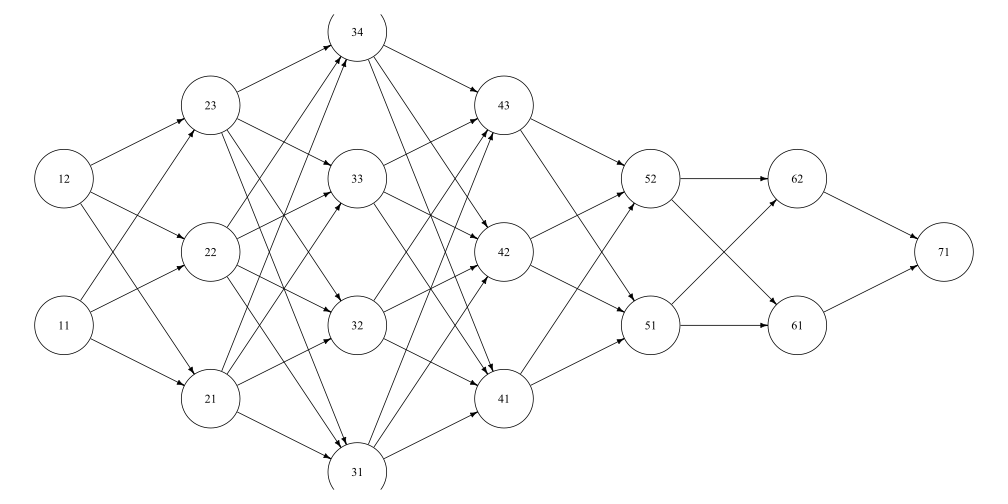
\includegraphics[trim={0 4.3cm 0 4.3cm}, width=\textwidth]{figures/nn.pdf}
  \caption{Neural network with four hidden layers}
  \label{fig:nn}
\end{figure}

A \textit{neural network} is a connected system of nodes and directed arcs, similar to a Bayesian network.
The differences between neural networks and Bayesian networks are that each node in a neural network consists of an activation function, a loss function, and an optimization algorithm, and each arc is assigned a weight based on its relative importance.

A \textit{deep feedforward neural network} is a neural network with an input layer, two or more hidden layers, and an output layer (Figure \ref{fig:nn}).
A deep feedforward neural network is comprised of many different functions, which approximate $\theta$ in the function $f(x;\theta)$ and form complex chains that map $x$ to $f(x;\theta)$.
Each chain is a function of the form $f_{i}(f_{i - 1}(f_{i - 2}(... (f_{i = 1}(x;\theta)))))$ where the maximum value of $i$ represents the depth of the network.
The output of the first hidden layer of the neural network, shown in Figure \ref{fig:nn}, is calculated using \ref{eq:nn1}.
%
\begin{equation}
  \label{eq:nn1}
  \left[
  \begin{matrix}
    x_{21} \\
    x_{22} \\
    x_{23} \\
  \end{matrix}
  \right] = g
  \left(
  \left[
  \begin{matrix}
    W_{10 \rightarrow 21} x_{10} + W_{11 \rightarrow 21} x_{11} + W_{12 \rightarrow 21} x_{12} \\
    W_{10 \rightarrow 22} x_{10} + W_{11 \rightarrow 22} x_{11} + W_{12 \rightarrow 22} x_{12} \\
    W_{10 \rightarrow 23} x_{10} + W_{11 \rightarrow 23} x_{11} + W_{12 \rightarrow 23} x_{12} \\
  \end{matrix}
  \right] + b_{1}
  \right)
\end{equation}

\noindent where \\
\indent $x_{ij} = $ output of neuron $ij$ \\
\indent $W_{ij \rightarrow (i + 1)k} = $ weight from the output of neuron $ij$ to the input of neuron $(i + 1)k$ \\
\indent $b_{i} = $ bias \\
\indent $g(x) = $ activation function \\

\noindent Similarly, the output of each hidden layer, shown in Figure \ref{fig:nn}, is calculated using \ref{eq:nn2}.
%
\begin{equation}
  \label{eq:nn2}
  \begin{split}
    &
    \left[
    \begin{matrix}
      x_{31} \\
      x_{32} \\
      x_{33} \\
      x_{34} \\
    \end{matrix}
    \right] = g
    \left(
    \left[
    \begin{matrix}
      W_{20 \rightarrow 31} x_{20} + W_{21 \rightarrow 31} x_{21} + W_{22 \rightarrow 31} x_{22} + W_{23 \rightarrow 31} x_{23} \\
      W_{20 \rightarrow 32} x_{20} + W_{21 \rightarrow 32} x_{21} + W_{22 \rightarrow 32} x_{22} + W_{23 \rightarrow 32} x_{23} \\
      W_{20 \rightarrow 33} x_{20} + W_{21 \rightarrow 33} x_{21} + W_{22 \rightarrow 33} x_{22} + W_{23 \rightarrow 33} x_{23} \\
      W_{20 \rightarrow 34} x_{20} + W_{21 \rightarrow 34} x_{21} + W_{22 \rightarrow 34} x_{22} + W_{23 \rightarrow 34} x_{23} \\
    \end{matrix}
    \right] + b_{2}
    \right) \\
    &
    \left[
    \begin{matrix}
      x_{41} \\
      x_{42} \\
      x_{43} \\
    \end{matrix}
    \right] = g
    \left(
    \left[
    \begin{matrix}
      W_{30 \rightarrow 41} x_{30} + W_{31 \rightarrow 41} x_{31} + W_{32 \rightarrow 41} x_{32} + W_{33 \rightarrow 41} x_{33} + W_{34 \rightarrow 41} x_{34} \\
      W_{30 \rightarrow 42} x_{30} + W_{31 \rightarrow 42} x_{31} + W_{32 \rightarrow 42} x_{32} + W_{33 \rightarrow 42} x_{33} + W_{34 \rightarrow 42} x_{34} \\
      W_{30 \rightarrow 43} x_{30} + W_{31 \rightarrow 43} x_{31} + W_{32 \rightarrow 43} x_{32} + W_{33 \rightarrow 43} x_{33} + W_{34 \rightarrow 43} x_{34} \\
    \end{matrix}
    \right] + b_{3}
    \right) \\
    &
    \left[
    \begin{matrix}
      x_{51} \\
      x_{52} \\
    \end{matrix}
    \right] = g
    \left(
    \left[
    \begin{matrix}
      W_{40 \rightarrow 51} x_{40} + W_{41 \rightarrow 51} x_{41} + W_{42 \rightarrow 51} x_{42} + W_{43 \rightarrow 51} x_{43} \\
      W_{40 \rightarrow 52} x_{40} + W_{41 \rightarrow 52} x_{41} + W_{42 \rightarrow 52} x_{42} + W_{43 \rightarrow 52} x_{43} \\
    \end{matrix}
    \right] + b_{4}
    \right)
  \end{split}
\end{equation}

\noindent The output of the last layer, shown in Figure \ref{fig:nn}, is calculated using \ref{eq:nn3}.
Unlike \ref{eq:nn1} and \ref{eq:nn2}, \ref{eq:nn3} uses a linear activation function, which is the same as having no activation function.
This allows the neural network to generate output that is positive or negative (Figure \ref{fig:relu}) \cite{goodfellow}.
%
\begin{equation}
  \label{eq:nn3}
  \left[
  \begin{matrix}
    x_{61}
  \end{matrix}
  \right] =
  \left[
  \begin{matrix}
    W_{50 \rightarrow 61} x_{50} + W_{51 \rightarrow 61} x_{51} + W_{52 \rightarrow 61} x_{52}
  \end{matrix}
  \right] + b_{5}
\end{equation}

\noindent Following \ref{eq:nn1}-\ref{eq:nn3} results in one forward pass of input through the neural network.
The vector output from \ref{eq:nn3} is then passed to a loss function, which for regression problems, is typically the \gls{mse}, shown in \ref{eq:mse1} \cite{chollet, goodfellow}.
%
\begin{equation}
  \label{eq:mse1}
  \mbox{MSE} = \frac{1}{n} \sum_{j = 1}^{n} (x_{observed_{j}} - x_{predicted_{j}})^2
\end{equation}

\noindent where \\
\indent $n = $ total number of variables that are observed or predicted \\
\indent $x = $ vector of observations or predictions \\

In this work, each neural network layer is densely (or fully) connected, and each hidden neuron uses a rectified linear unit activation function, which is a piecewise function that returns $x$ if $x > 0$ and 0 if $x \leq 0$ (Figure \ref{fig:relu}).

\vspace{+0.6cm}
\begin{figure}[H]
  \centering
  \includegraphics[scale=1]{figures/relu.png}
  \caption{Rectified linear unit (ReLU) activation function}
  \label{fig:relu}
\end{figure}

\noindent A simplified equation for a deep feedforward neural network with four hidden layers is shown in \ref{eq:nn4} \cite{goodfellow}.
%
\begin{equation}
  \label{eq:nn4}
  f(x; W, b) = W_{5}^{\top} \prod_{i = 1}^{4} \left( max \{ 0, W_{i}^{\top} x_{i} + b_{i} \} \right) + b_{5}
\end{equation}

\noindent where \\
\indent $W_{5}^{\top} + b_{5} = $ row vector mapping the last hidden layer to the output layer \\
\indent $max \{ 0, W_{i}^{\top} x_{i} + b_{i} \} = $ row vector mapping adjacent input and hidden layers \\

\noindent \ref{eq:mse1} is the general form of the \gls{mse} equation.
Substituting $x_{predicted_{i}}$ for the right side of \ref{eq:nn4} yields \ref{eq:mse2}.
%
\begin{equation}
  \label{eq:mse2}
  \mbox{MSE} = \frac{1}{n} \sum_{j = 1}^{n} \left( y_{j} - \left[ W_{5}^{\top} \prod_{i = 1}^{4} \left( max \{ 0, W_{i}^{\top} x_{i} + b_{i} \} \right) + b_{5} \right]_{j} \right)^{2}
\end{equation}

\noindent The output from the \gls{mse} loss function (\ref{eq:mse2}) is passed to the optimization algorithm, which updates parameters ($\theta$) by implementing the backpropagation algorithm \cite{goodfellow}.
The backpropagation algorithm is the backbone of a neural network and applies the chain rule to compute gradients (i.e., the vector of partial derivatives with respect to $\theta$ evaluated at time step \textit{i} \ref{alg:adamax}) and update parameters ($\theta$) \cite{goodfellow}.
These parameters ($\theta$) are also referred to as the weights ($W$) and biases ($b$) of the neural network in \ref{eq:nn1}-\ref{eq:nn4}.
In this work, the Adamax optimization algorithm (Algorithm \ref{alg:adamax}) is used to update parameters ($\theta$) \cite{kingma}.
Adamax is a variant of Adam (Algorithm \ref{alg:adam}) \cite{kingma} based on the exponentially weighted infinity norm, which takes the place of the bias-corrected first and second moment estimates \cite{kingma}.

\vspace{+0.6cm}
\begin{algorithm}[H]
  \centering
  \caption{Adamax optimization algorithm \cite{kingma}}
  \label{alg:adamax}
  \begin{algorithmic}
    \STATE \textbf{Require}: $\alpha = $ step size
    \STATE \textbf{Require}: $\beta_{1}, \beta_{2} \in \left[ 0, 1 \right) = $ exponential decay rates for the moment estimates
    \STATE \textbf{Require}: $f(x; \theta) = $ loss function with parameters $\theta$
    \STATE \textbf{Require}: $\theta_{0} = $ initial parameter vector
    \STATE $m_{0} \leftarrow 0$ (initialize first moment vector)
    \STATE $u_{0} \leftarrow 0$ (initialize exponentially weighted infinity norm)
    \STATE $i \leftarrow 0$ (initialize first iteration)
    \STATE \textbf{while} $\theta_{i}$ not converged \textbf{do}
    \STATE \hspace{\algorithmicindent} $i \leftarrow i + 1$
    \STATE \hspace{\algorithmicindent} $g_{i} \leftarrow \bigtriangledown_{\theta} f_{i} (\theta_{i - 1})$ (get gradients from loss function at time step $i$)
    \STATE \hspace{\algorithmicindent} $m_{i} \leftarrow \beta_{1} \cdot m_{i - 1} + (1 - \beta_{1}) \cdot g_{i}$ (update biased first moment estimate)
    \STATE \hspace{\algorithmicindent} $u_{i} \leftarrow max(\beta_{2} \cdot u_{t - 1}, |g_{i}|)$ (update exponentially weighted infinity norm)
    \STATE \hspace{\algorithmicindent} $\theta_{i} \leftarrow \theta_{t - 1} - (\alpha / (1 - \beta_{1}^{i})) \cdot m_{i} / u_{i}$ (update parameters)
    \STATE \textbf{return} $\theta_{i}$
  \end{algorithmic}
\end{algorithm}

\vspace{+0.6cm}
\begin{algorithm}[H]
  \centering
  \caption{Adam optimization algorithm \cite{kingma}}
  \label{alg:adam}
  \begin{algorithmic}
    \STATE \textbf{Require}: $\alpha = $ step size
    \STATE \textbf{Require}: $\beta_{1}, \beta_{2} \in \left[ 0, 1 \right) = $ exponential decay rates for the moment estimates
    \STATE \textbf{Require}: $f(x; \theta) = $ loss function with parameters $\theta$
    \STATE \textbf{Require}: $\theta_{0} = $ initial parameter vector
    \STATE $m_{0} \leftarrow 0$ (initialize first moment vector)
    \STATE $v_{0} \leftarrow 0$ (initialize second moment vector)
    \STATE $i \leftarrow 0$ (initialize first iteration)
    \STATE \textbf{while} $\theta_{i}$ not converged \textbf{do}
    \STATE \hspace{\algorithmicindent} $i \leftarrow i + 1$
    \STATE \hspace{\algorithmicindent} $g_{i} \leftarrow \bigtriangledown_{\theta} f_{i} (\theta_{i - 1})$ (get gradients from loss function at time step $i$)
    \STATE \hspace{\algorithmicindent} $m_{i} \leftarrow \beta_{1} \cdot m_{i - 1} + (1 - \beta_{1}) \cdot g_{i}$ (update biased first moment estimate)
    \STATE \hspace{\algorithmicindent} $v_{i} \leftarrow \beta_{2} \cdot v_{i - 1} + (1 - \beta_{2}) \cdot g_{i}^{2}$ (update biased second moment estimate)
    \STATE \hspace{\algorithmicindent} $\hat m_{i} \leftarrow m_{i} / (1 - \beta_{1}^{i})$ (calculate bias-corrected first moment estimate)
    \STATE \hspace{\algorithmicindent} $\hat v_{i} \leftarrow v_{i} / (1 - \beta_{2}^{i})$ (calculate bias-corrected second moment estimate)
    \STATE \hspace{\algorithmicindent} $\theta_{i} \leftarrow \theta_{i - 1} - \alpha \cdot \hat m_{i} / (\sqrt{\hat v_{i}} + \epsilon)$ (update parameters)
    \STATE \textbf{return} $\theta_{i}$
  \end{algorithmic}
\end{algorithm}
